%%%%%%%%%%%%%%%%%%%%%%%%%%%%%%%%%%%%%%%%%%%%%%%%%%%%%%%%%%%%%%%%%%%%%%%%%%%%
%% Focused manuscript: one-round, verifiable range aggregation.
%%
%% THIS IS A SKELETON FOR THE AUTHORS TO WRITE.
%%  - Every grey box (\para{...}{...}) is one paragraph to be written by the
%%    authors: the first argument is the point the paragraph must make, the
%%    second the facts and numbers it may use. Delete the box when the
%%    paragraph is written.
%%  - Equations, definitions, theorem statements, the algorithm, figures and
%%    tables are filled in; reword them freely but keep the mathematics.
%%  - Copy numbers only from NUMBERS.md (generated from results/*.json).
%%  - Read OUTLINE.md first: argument, style rules, what was cut, checklist.
%% Build: pdflatex -> bibtex -> pdflatex -> pdflatex
%%%%%%%%%%%%%%%%%%%%%%%%%%%%%%%%%%%%%%%%%%%%%%%%%%%%%%%%%%%%%%%%%%%%%%%%%%%%
\documentclass[a4paper,fleqn]{cas-sc}

\usepackage[numbers,sort&compress]{natbib}
\usepackage{algorithm}
\usepackage{algpseudocode}
\usepackage[most]{tcolorbox}
\setlength{\emergencystretch}{3em}
\providecommand{\checkmark}{\ensuremath{\surd}}
\makeatletter\let\inputtbl\@@input\makeatother

% ---- writing placeholders: delete each box once its paragraph is written ----
\newif\ifskeleton \skeletontrue          % \skeletonfalse hides all boxes
\newtcolorbox{parabox}{breakable,colback=black!4,colframe=black!25,boxrule=0.4pt,
  arc=1pt,left=4pt,right=4pt,top=2pt,bottom=2pt,fontupper=\small}
\newcommand{\para}[2]{\ifskeleton\begin{parabox}\textbf{Write:} #1
  \par\smallskip\textit{Use:} #2\end{parabox}\fi}

\newtheorem{theorem}{Theorem}
\newtheorem{lemma}{Lemma}
\newtheorem{remark}{Remark}
\newdefinition{definition}{Definition}
\newproof{pf}{Proof}

% Shared by the LaTeX build (manuscript.tex) and the Word build (build_docx.py).
\newcommand{\negl}{\mathsf{negl}}
\newcommand{\PPT}{\mathrm{PPT}}
\newcommand{\Real}{\mathbf{Real}}
\newcommand{\Ideal}{\mathbf{Ideal}}
\newcommand{\Leak}{\mathcal{L}}
\newcommand{\Sim}{\mathcal{S}}
\newcommand{\Adv}{\mathcal{A}}
\newcommand{\cind}{\approx_c}
\newcommand{\Gen}{\mathsf{Gen}}
\newcommand{\Eval}{\mathsf{Eval}}
\newcommand{\Enc}{\mathsf{Enc}}
\newcommand{\Dec}{\mathsf{Dec}}
\newcommand{\advPRF}{\mathrm{Adv}^{\mathrm{prf}}}
\newcommand{\advDPF}{\mathrm{Adv}^{\mathrm{dpf}}}
\newcommand{\advCPA}{\mathrm{Adv}^{\mathrm{cpa}}}
\newcommand{\bplus}{\boxplus}
\newcommand{\bdot}{\boxdot}


\begin{document}
\let\WriteBookmarks\relax
\def\floatpagepagefraction{1}
\def\textpagefraction{.001}

\shorttitle{Verifiable range aggregation over encrypted multi-cloud data}
\shortauthors{M. M. Islam et~al.}

% Title options (choose one; see OUTLINE.md):
%  (a) One-round verifiable range aggregation over encrypted data replicated
%      across non-colluding clouds
%  (b) Oblivious and verifiable range queries over homomorphically encrypted
%      IoT data in multi-cloud storage
\title[mode=title]{One-round verifiable range aggregation over encrypted data
replicated across non-colluding clouds}

\author[1]{Md Mazharul Islam}[orcid=0000-0001-6225-1487]
\cormark[1]
\ead{mazharul.islam1@northsouth.edu}
\credit{To be completed by the authors}

\author[1]{Mubasshir Ahmed}[orcid=0000-0002-7502-3835]
\ead{mubasshir.ahmed@northsouth.edu}
\credit{To be completed by the authors}

\author[1]{Md Redowan Zaman Anik}
\ead{redowan.anik@northsouth.edu}
\credit{To be completed by the authors}

\affiliation[1]{organization={Department of Electrical and Computer
    Engineering, North South University},
    addressline={Plot 15, Block B, Bashundhara R/A},
    city={Dhaka},
    postcode={1229},
    country={Bangladesh}}

\cortext[cor1]{Corresponding author.}

\begin{abstract}
\textbf{[Write:]} One paragraph, at most 200 words, no citations, no symbols except $n$
and $d$. Order: the setting (IoT data encrypted and stored at several clouds;
analysts want sums and counts over ranges); what existing designs cannot do
(hide which records a range selects while the clouds compute on encrypted data
and detect a wrong answer, without the clouds talking to each other); what we
propose (one sentence); the two technical ideas (one sentence each); the
evaluation and its three headline results; one closing sentence on what this
enables. \textbf{[Use:]} Two real IoT datasets, 405{,}184 and 420{,}370 records. A verified
range query costs 0.68--1.19\,s per cloud on one thread, the same for one
minute as for the whole timeline; one 132\,kB reply per cloud; about 5\,kB of
keys per cloud against a 44\,MB encrypted query for one server. No tampered
answer accepted in 1{,}000 synthetic and 500 real-data trials. Hidden from any
$n-1$ colluding clouds: the range, the matching records, their number and the
result.
\end{abstract}

\begin{highlights}
\item To be written by the authors: 3--5 bullets, at most 85 characters each
\end{highlights}

\begin{keywords}
Homomorphic encryption \sep
Distributed point functions \sep
Range aggregation \sep
Verifiable computation \sep
Multi-cloud storage \sep
Internet of Things
\end{keywords}

\maketitle

% ===========================================================================
\section{Introduction}
\label{sec:intro}

\para{The setting, concretely. IoT data are collected by one organisation,
encrypted, and stored at several cloud providers; other parties query them.
Give one running example and keep it through the paper.}{Example: a city's air
monitoring office stores readings at three clouds; a health agency asks how many
hours carbon monoxide stayed in its top bands at one site last month. Cite
\citep{atzori2010internet} for IoT data volume and
\citep{petcu2013multicloud,grozev2014intercloud} for multi-cloud storage.}

\para{Why encryption alone is not enough: the clouds see which records a query
touches (the access pattern), and known attacks turn that into the data.}{Cite
\citep{islam2012access,cash2015leakage,grubbs2017leakage}. One sentence on
single-server homomorphic encryption hiding the query but needing a query as
large as the data's index (we measure 44\,MB for our cube).}

\para{The gap. Splitting the query across non-colluding clouds hides the access
pattern, but existing multi-server systems either compute on plaintext replicas,
need an honest majority and server-to-server rounds, or stop at retrieval; and
none detects a wrong answer from colluding clouds at no extra homomorphic cost.
State the three requirements as a list: (R1) privacy against any $n-1$ colluding
clouds; (R2) one round, no communication between clouds; (R3) data encrypted
once under the owner's key; plus (R4) the analyst detects a wrong
answer.}{Splinter \citep{splinter} (plaintext replicas), Waldo \citep{waldo}
(honest majority, server interaction), Obscure \citep{gupta2020obscure} (honest
majority, one-dimensional ranges), Hafiz et al.\ \citep{hafiz2024private}
(plaintext replicas, no ranges). Details go to Section~\ref{sec:related}, not
here.}

\para{Our approach in plain words, before any symbol. The owner precomputes
running totals (summed-area tables) of the data cube and encrypts them; any box
then equals a signed sum of $2^d$ table entries; the analyst hides those $2^d$
positions in distributed point function keys, one share per cloud; each cloud
multiplies its share into the encrypted table and returns one ciphertext; a
second set of keys carries a fresh secret number so that the analyst can check
the answer.}{Refer to Fig.~\ref{fig:system} and Fig.~\ref{fig:rangeidea}.}

\para{Contributions, as a list of three. Each item one or two sentences; no
section numbers.}{(1) One-round range aggregation over encrypted summed-area
tables with dummy-padded corner keys: cost independent of the range and of the
number of records; the clouds never see a record's coordinates. (2) A
per-query check carried inside the keys: a wrong answer is accepted with
probability at most $1/(p-1)$ plus the DPF advantage, against any $n-1$
deviating clouds, with no stored key and no extra homomorphic product; it gives
no protection if one server holds the whole query, which is why it needs the
split. (3) Proofs, an implementation on OpenFHE, and an evaluation on two real
IoT datasets against a per-cell baseline and a single-server baseline on the
same machine.}

\para{What is borrowed, credited plainly.}{The $2^d$ decomposition of a box is
Boyle, Gilboa and Ishai's \citep[Cor.~3.4]{boyle2016function}; we apply it to an
encrypted table instead of to the query predicate. Summed-area tables are
\citep{crow1984summed,ho1997range}. A one-time MAC key chosen by the client is
in PVODTE \citep{li2026silent}; we deliver it inside DPF outputs. Searches of
the venues listed in OUTLINE.md found no system with (R1)--(R4); say ``to our
knowledge'', not ``first''.}

\para{Organisation, one short paragraph.}{Sections~\ref{sec:related}--\ref{sec:conclusion}.}

% ===========================================================================
\section{Related work}
\label{sec:related}

\para{Multi-server private queries: what each closest system does, and the one
requirement it does not meet. One or two sentences per system.}{Splinter
\citep{splinter}: function secret sharing over public cleartext replicas;
one-dimensional intervals; no result verification. Waldo \citep{waldo}:
secret-shared time series, three parties, honest majority, server interaction,
malicious security. Obscure \citep{gupta2019obscure,gupta2020obscure}: Shamir
shares, non-communicating servers, needs $2l+1$ servers for a length-$l$
predicate, honest majority, ranges in one dimension. Hafiz et al.\
\citep{hafiz2024private}: one-round aggregates by information-theoretic PIR over
plaintext copies, no range predicates. These four are read in full
(docs/NOVELTY\_SEARCH.md).}

\para{Range aggregation over encrypted or private data at one server.}{ARQ
\citep{espiritu2022arq}: structured encryption, query-dependent leakage. HADES
\citep{liu2025hades}: one round over a single provider's plaintext data; reports
more than fifteen hours for one-round homomorphic processing of a million
encrypted records. Timecrypt \citep{timecrypt} and Zeph \citep{zeph}: encrypted
time series, the queried interval is revealed. Prefix sums for range sums:
\citep{ho1997range,crow1984summed}. FSS for intervals: \citep{boyle2016function}.}

\para{Verifying answers.}{Verifiable DPFs \citep{decastro2022lightweight} and
access control for FSS \citep{pacl,ji2023finegrained} protect against a
malicious client, not malicious servers. Verifiable homomorphic secret sharing
\citep{choudhuri2024vehss}. PVODTE \citep{li2026silent}: client-chosen one-time
MAC key sent under HSS to two servers, one malicious server. SPDZ-style MACs
\citep{damgard2012spdz}.}

\begin{table*}[pos=t,width=\textwidth]
\caption{Systems closest to ours ($\checkmark$ yes, $\circ$ partly, $\times$ no).}
\label{tab:compare}
\centering
\footnotesize
\setlength{\tabcolsep}{4pt}
\begin{tabular*}{\tblwidth}{@{\extracolsep{\fill}}lccccc@{}}
\toprule
System & Data at the servers & Range aggregates & Colluding servers tolerated & Server-to-server rounds & Detects wrong answers \\
\midrule
Splinter \citep{splinter} & plaintext copies & $\circ$ (1-D) & $n-1$ & none & $\times$ \\
Waldo \citep{waldo} & secret-shared & $\checkmark$ & 1 of 3 & yes & $\checkmark$ \\
Obscure \citep{gupta2020obscure} & Shamir-shared & $\circ$ (1-D) & minority & none & optional \\
Hafiz et al.\ \citep{hafiz2024private} & plaintext copies & $\times$ & $n-1$ & none & $\circ$ \\
HADES \citep{liu2025hades} & plaintext, one server & $\checkmark$ & n/a & n/a & $\times$ \\
ARQ \citep{espiritu2022arq} & encrypted, one server & $\checkmark$ (with leakage) & n/a & n/a & $\times$ \\
\midrule
\textbf{This work} & encrypted copies & $\checkmark$ ($d$-D) & $n-1$ & none & $\checkmark$ \\
\bottomrule
\end{tabular*}
\end{table*}

% ===========================================================================
\section{Model and building blocks}
\label{sec:model}

\para{The three parties and what each holds, matching
Fig.~\ref{fig:system}. Use full words (data owner, cloud, analyst); define no
abbreviations.}{The data owner holds the homomorphic secret key $sk$ and builds
the encrypted tables. Each of $n$ clouds stores a copy of the encrypted tables
and the public evaluation keys, never decrypts. The analyst receives $sk$ from
the owner, issues queries and combines replies.}

\begin{figure*}[pos=t,width=\textwidth]
\centering
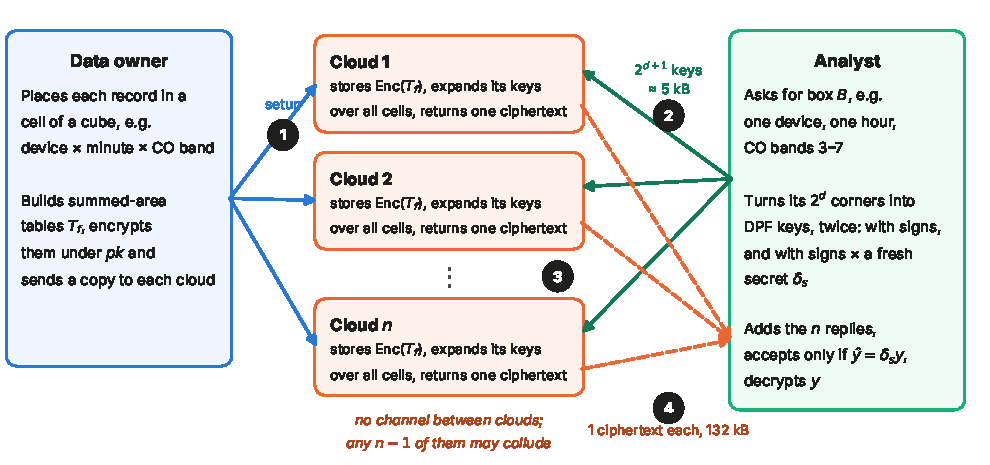
\includegraphics[width=\textwidth]{figures/fig_system.pdf}
\caption{System overview: (1) the owner stores encrypted summed-area tables at
$n$ clouds; (2) the analyst sends each cloud its share of the query as DPF
keys; (3) each cloud returns one ciphertext; (4) the analyst adds the replies,
checks and decrypts.}
\label{fig:system}
\end{figure*}

\para{Data cubes and aggregate templates, defined before use.}{A cube has $d$
ordered attributes of sizes $s_1,\dots,s_d$ and $M=\prod_k s_k$ cells; each
record $i$ lies in one cell $c(i)$. A template $f$ fixes what record $i$
contributes, $w_f[i]\,m_i$ (count: $1$; sum: the reading; sum of squares: its
square). A range query asks for $\sum_{i:\,c(i)\in B}w_f[i]\,m_i$ over a box
$B=\prod_k[\mathit{lo}_k,\mathit{hi}_k]$. Templates and cubes are registered at
setup.}

\para{Threat model, in four sentences: who is corrupted, how, what must stay
hidden, what is out of scope.}{Static PPT adversary corrupting up to $t=n-1$
clouds. For privacy, the coalition follows the protocol and pools its views
over adaptively chosen queries; it must learn nothing beyond the leakage of
Section~\ref{sec:security} (not the box, the matching records, their number or
the result). For correctness, the coalition may return anything; the analyst
must reject a wrong answer. The owner and analyst are honest; channels are
authenticated; side channels other than message sizes, and collusion between
the analyst and a cloud, are out of scope.}

\para{Building blocks: DPF and BFV, with only what the paper uses.}{An $n$-party
DPF \citep{gilboa2014distributed,boyle2015function,boyle2016function} for point
functions $f_{\alpha,\beta}:[M]\to\mathbb{Z}_p$: $\Gen(1^\lambda,\alpha,\beta)$
gives keys $\kappa_1,\dots,\kappa_n$ with $\sum_j\Eval(\kappa_j,x)=f_{\alpha,\beta}(x)$;
any $n-1$ keys hide $(\alpha,\beta)$ up to $\advDPF$. Two-party keys have
$O(\lambda\log M)$ bits. Leveled BFV \citep{fan2012somewhat} over
$\mathbb{Z}_p$, IND-CPA with advantage $\advCPA$; $\bplus$ adds ciphertexts and
$\bdot$ multiplies a plaintext into a ciphertext; $\ell$ slots in two rows of
$\ell/2$ \citep{halevi2014algorithms}. Table~\ref{tab:notation}.}

\begin{table}[pos=htbp]
\caption{Notation.}
\label{tab:notation}
\centering
\footnotesize
\begin{tabular}{@{}ll@{}}
\toprule
Symbol & Meaning \\
\midrule
$n$ & number of clouds; up to $n-1$ may collude \\
$d$, $s_k$, $M$ & cube dimension, size of attribute $k$, number of cells \\
$C_f$, $T_f$ & cell aggregates and their summed-area table \\
$B$, $\kappa_\sigma(B)$, $\beta_\sigma$ & box; its corner $\sigma\in\{0,1\}^d$; that corner's sign or $0$ \\
$e_j$ & sum of cloud $j$'s key evaluations over all cells \\
$\delta_s$ & per-query secret of the check, uniform on $\mathbb{Z}_p^{*}$ \\
$p$, $\ell$ & plaintext modulus (also the DPF output group); BFV slots \\
\bottomrule
\end{tabular}
\end{table}

% ===========================================================================
\section{Construction}
\label{sec:construction}

\subsection{Computing on a shared selection}
\label{sec:oha}

\para{The core operation: each cloud multiplies its own share of the selection
into the encrypted table, so the selection is never assembled anywhere.}{State
Eq.~\eqref{eq:contract} and Lemma~\ref{lem:compat}. One sentence: using one
modulus $p$ for the DPF outputs and the BFV plaintexts is what makes the shares
add up correctly; two independent libraries with different moduli silently give
wrong answers.}

\begin{equation}
\label{eq:contract}
\mathrm{ct}_j=\bplus_{x\in[M]} e_j[x]\bdot\Enc_{pk}(T_f[x]),\qquad
\Dec\Big(\bplus_{j\in[n]}\mathrm{ct}_j\Big)=\sum_{x}\Big(\sum_j e_j[x]\Big)T_f[x].
\end{equation}

\begin{lemma}[Algebraic compatibility]
\label{lem:compat}
If the DPF output group and the BFV plaintext ring are the same $\mathbb{Z}_p$,
then $\bplus_j\mathrm{ct}_j$ decrypts to $\sum_x e[x]\,T_f[x]\bmod p$ with
$e=\sum_je_j$, except with the probability that decryption fails.
\end{lemma}
\begin{pf}
$\bdot$ and $\bplus$ are homomorphisms of $\mathbb{Z}_p$-modules, so summation
commutes with decryption. The noise added by multiplying with a uniform
element of $\mathbb{Z}_p$ is bounded by the parameters of
Section~\ref{sec:setup}; Section~\ref{sec:correct} checks it on every query. \qed
\end{pf}

\subsection{Range queries over summed-area tables}
\label{sec:range}

\para{Define the tables and state inclusion--exclusion; then explain dummy keys
and why every query sends exactly $2^d$ keys; walk through
Fig.~\ref{fig:rangeidea}.}{$C_f[c]=\sum_{i:\,c(i)=c}w_f[i]\,m_i$;
$T_f[c]=\sum_{c'\le c}C_f[c']$ (coordinate-wise $\le$), flattened to $M$
entries and encrypted in slot row 0, with a copy in row 1. Corner
$\kappa_\sigma(B)$ takes $\mathit{lo}_k-1$ where $\sigma_k=1$ and
$\mathit{hi}_k$ elsewhere. A corner with a coordinate $-1$ lies outside the
cube; the analyst replaces it by a dummy key with output $0$ at a random cell.
DPF keys hide the output as well as the point, so a box at the edge looks like
any other.}

\begin{equation}
\label{eq:ie}
\sum_{c\in B}C_f[c]=\sum_{\sigma\in\{0,1\}^d}(-1)^{|\sigma|}\,T_f[\kappa_\sigma(B)],
\end{equation}

\begin{figure}[pos=htbp]
\centering
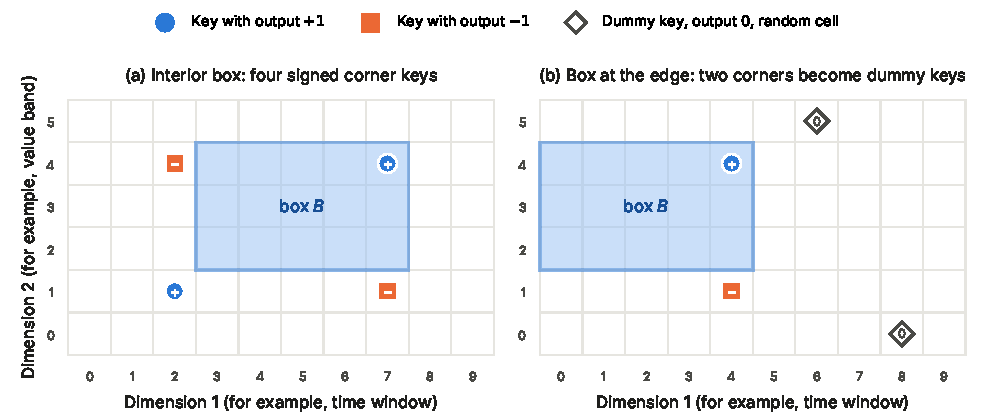
\includegraphics[width=\linewidth]{figures/fig_range_idea.pdf}
\caption{A two-dimensional box as signed corners of the summed-area table. At
the edge of the cube, dummy keys keep the number of keys fixed.}
\label{fig:rangeidea}
\end{figure}

\para{Why prefix sums on the data side instead of interval keys. Two or three
sentences.}{BGI interval keys need the clouds to hold each record's coordinates
in the clear; over encrypted records the coordinates are the sensitive part. A
dense encrypted table over all $M$ cells keeps them hidden; the price is that
cubes are registered in advance and cost grows with $M$.}

\subsection{The per-query check}
\label{sec:check}

\para{The check in three steps: (i) a fixed stored key fails against a cloud
that changes both slot rows consistently (give the example of scaling its
share); (ii) the fix: a fresh secret $\delta_s$ per query, carried in a second
set of keys with outputs $\delta_s\beta_\sigma$, placed in slot row 1 of the
same plaintexts, so no extra homomorphic product; (iii) accept only if
$\hat y=\delta_s y$.}{Theorem~\ref{thm:tamper}; Table~\ref{tab:tamper} shows
(i) failing and (ii) working.}

\para{Why the check needs the split (Remark~\ref{rem:single}).}{A single
server that holds encryptions of the whole selection and of its
$\delta_s$-multiple can alter the table in both rows alike and the check
passes; with two clouds the same alteration is caught. Exercised by
tests/test\_session\_mac.py.}

\begin{remark}
\label{rem:single}
The check relies on no cloud holding the whole selection. A single server
holding $\Enc(e)$ and $\Enc(\delta_s e)$ can replace $T_f$ by any $T'_f$ in both
slot rows and return $\Enc(\langle e,T'_f\rangle,\delta_s\langle
e,T'_f\rangle)$, which passes.
\end{remark}

\subsection{The protocol}
\label{sec:protocol}

\para{Walk through Algorithm~\ref{alg:range} and state the cost.}{Per cloud:
$2^{d+1}$ full-domain DPF evaluations over $M$ cells, $\lceil kM/(\ell/2)\rceil$
plaintext-ciphertext products for $k$ templates, $\log_2(\ell/2k)$ rotations;
upload $2^{d+1}$ keys of $O(\lambda\log M)$ bits; reply one ciphertext. Nothing
depends on the box or on the number of records. A single-keyword aggregate is
the case $d=1$ with a box of one cell (mention in one sentence; the
keyword-search machinery of earlier versions is not part of this paper).}

\begin{algorithm}[t]
\footnotesize
\caption{Verified range query on a registered cube.}
\label{alg:range}
\begin{algorithmic}[1]
\Statex \textbf{Setup} at the data owner, once per cube and template $f$
\State $C_f[c]\gets\sum_{i:\,c(i)=c}w_f[i]\,m_i$; \ $T_f[c]\gets\sum_{c'\le c}C_f[c']$
\State pack $T_f$ in slot row 0 with a copy in row 1, encrypt under $pk$, send to every cloud
\Statex \textbf{Query} at the analyst, for box $B$
\State $\delta_s\gets\mathbb{Z}_p^{*}$ \Comment{fresh per query}
\ForAll{$\sigma\in\{0,1\}^d$}
  \State $c\gets\kappa_\sigma(B)$; \ $\beta\gets(-1)^{|\sigma|}$
  \State \textbf{if} $c$ lies outside the cube \textbf{then} $c\gets$ random cell; $\beta\gets0$ \Comment{dummy}
  \State $(\kappa_{\sigma,1},\dots,\kappa_{\sigma,n})\gets\Gen(1^\lambda,c,\beta)$; \
         $(\hat\kappa_{\sigma,1},\dots,\hat\kappa_{\sigma,n})\gets\Gen(1^\lambda,c,\delta_s\beta)$
\EndFor
\State send $\{\kappa_{\sigma,j},\hat\kappa_{\sigma,j}\}_\sigma$ to cloud $j$
\Statex \textbf{Answer} at cloud $j$
\State $e_j\gets\sum_\sigma\Eval(\kappa_{\sigma,j},\cdot)$ and
       $\hat e_j\gets\sum_\sigma\Eval(\hat\kappa_{\sigma,j},\cdot)$ over all $M$ cells
\State $\mathrm{ct}_j\gets\bplus_c E_{j,c}\bdot\Enc(T_f)_c$, where $E_{j,c}$ holds chunk $c$ of $e_j$ in row 0 and of $\hat e_j$ in row 1
\State sum within each row by rotations; \Return $\mathrm{ct}_j$ \Comment{one ciphertext}
\Statex \textbf{Combine} at the analyst
\State $(y,\hat y)\gets$ slots $(0,\ell/2)$ of $\Dec\big(sk,\bplus_j\mathrm{ct}_j\big)$
\State \textbf{if} $\hat y\neq\delta_s y$ \textbf{then} reject \textbf{else} \Return $y$
\end{algorithmic}
\end{algorithm}

% ===========================================================================
\section{Security}
\label{sec:security}

\para{What leaks, in words, then Definition~\ref{def:sec}.}{Setup leakage: $n$,
$p$, $\ell$, the cubes' sizes $(s_1,\dots,s_d)$, the number of templates and of
ciphertexts. Query leakage: which cube is queried and whether the check is
used (this fixes the number of keys). Not leaked: the box, the matching
records, their number, the result.}

\begin{definition}[Security against $t$ colluding clouds]
\label{def:sec}
In $\Real$, the adversary chooses the data and a coalition $C$ of at most $t$
clouds, receives the coalition's stored state, and adaptively issues $Q$ range
queries, receiving after each the coalition's keys and replies. In $\Ideal$, a
simulator produces the same view from the setup leakage and, for each query,
the cube queried and whether it is checked. The scheme is secure if for every
$\PPT$ adversary a $\PPT$ simulator makes the two views indistinguishable up to
$\negl(\lambda)$.
\end{definition}

\begin{theorem}[Correctness]
\label{thm:correct}
If $w_f[i]\,m_i\ge0$ for all records and the cube's total
$\sum_iw_f[i]\,m_i$ is below $p$, a query on box $B$ returns
$\sum_{i:\,c(i)\in B}w_f[i]\,m_i$, except with the probability that decryption
fails, and honest replies pass the check.
\end{theorem}
\begin{pf}[Proof sketch]
DPF correctness gives $\sum_je_j=\sum_\sigma\beta_\sigma u_{\kappa_\sigma(B)}$,
so by Lemma~\ref{lem:compat} the combined reply decrypts to
$\sum_\sigma\beta_\sigma T_f[\kappa_\sigma(B)]\bmod p$, which
Eq.~\eqref{eq:ie} turns into the box aggregate. That value lies in $[0,p)$,
so reduction modulo $p$ loses nothing although single terms are negative.
Row 1 decrypts to $\delta_s$ times row 0. Full proof: Supplementary S1. \qed
\end{pf}

\begin{theorem}[Privacy against $n-1$ colluding clouds]
\label{thm:sec}
If $(\Gen,\Eval)$ is an $(n{-}1)$-private DPF and BFV is IND-CPA, the scheme is
secure against $t=n-1$ colluding clouds in the sense of
Definition~\ref{def:sec}, with distinguishing advantage at most
\[
Q\,2^{d_{\max}+1}\,\advDPF+m\,\advCPA ,
\]
where $d_{\max}$ is the largest cube dimension and $m$ the number of ciphertexts
the coalition stores.
\end{theorem}
\begin{pf}[Proof sketch]
Hybrids replace (1) every DPF key the coalition receives, dummy and
$\delta_s$-carrying keys included, by simulated keys, which hide both point
and output; (2) every stored ciphertext by an encryption of $0$. Each reply is
a deterministic function of a cloud's keys and stored state, so the simulator
recomputes it. Full proof: Supplementary S2. \qed
\end{pf}

\begin{theorem}[Detection of wrong answers]
\label{thm:tamper}
Let up to $n-1$ clouds return arbitrary replies computed from their views,
with at least one cloud honest and $\delta_s$ known only to the analyst. The
analyst accepts an output $y'\neq y$, where $y$ is the correct answer, with
probability at most $1/(p-1)+2^d\,\advDPF$ per query.
\end{theorem}
\begin{pf}[Proof sketch]
Write the decrypted slots as $y'=y-y_C+r_0$ and
$\hat y'=\delta_sy-\hat y_C+r_1$, where $(r_0,r_1)$ is what the coalition
returned and $(y_C,\hat y_C)$ what it would have returned honestly; all are
functions of its view. The analyst accepts iff
$r_1-\hat y_C=\delta_s(y'-y)$. Replacing the coalition's $\delta_s$-carrying
keys by keys for an independent scalar changes this probability by at most
$2^d\advDPF$; then the view is independent of $\delta_s$, and as $y'\neq y$ at
most one of the $p-1$ values of $\delta_s$ satisfies the equation. Full proof:
Supplementary S3. \qed
\end{pf}

\para{What the theorems do not give, two or three sentences.}{No guaranteed
output (a cloud can force a rejection); an analyst who reveals its rejections
leaks up to one bit per query; privacy is proved for semi-honest clouds, but a
deviating coalition sees the same view, since clouds never interact. The bound
is set by $p\approx2^{36}$; $r$ independent scalars give $(p-1)^{-r}+r\,2^d\advDPF$
(not implemented).}

\para{Why not secret-share the data instead of encrypting it, one paragraph,
pointing to Supplementary S4.}{Under (R1)--(R3), answering over additive shares
of the data needs cross terms no cloud holds; a scheme that avoided this would
give single-server PIR, which needs public-key cryptography
\citep{dicrescenzo2000single,kushilevitz1997replication}. So the homomorphic
layer is not avoidable under these requirements.}

% ===========================================================================
\section{Implementation and setup}
\label{sec:setup}

\para{Implementation and parameters.}{Python reference implementation driving
OpenFHE's C++ kernels \citep{openfhe}; two-party GGM-tree DPF with fixed-key
AES-128 \citep{boyle2016function}; BFV with $p=68{,}724{,}326{,}401$ (37-bit
prime, $p\equiv1\bmod2^{17}$), ring dimension $8{,}192$, depth 1, 128-bit
security. The DPF output group and the plaintext ring are one modulus object
in the code. Tests compare range answers with brute force for $d\le3$ and
$n\le3$, and include failure controls (a flipped corner sign must give a wrong
answer). Say whether the code is available and on what terms.}

\para{Datasets and cubes.}{Environmental Sensor Telemetry
\citep{stafford_2020_environmental}: 405{,}184 records; cube device (3) $\times$
minute (11{,}523) $\times$ CO decile band (10), $M=345{,}690$. Beijing
Multi-Site Air Quality \citep{chen2019beijing}: 420{,}370 hourly records with
a temperature; cube site (12) $\times$ day (1{,}461) $\times$ PM$_{2.5}$ band
(10 deciles and one for missing), $M=192{,}852$. Templates: count and sum of
temperature in hundredths of a degree; Beijing temperatures are shifted by
$+50\,^\circ$C to keep them non-negative (Theorem~\ref{thm:correct}). Queries
fix one device or site, a window of $L$ minutes or days and bands 3--7.}

\para{Machines and method.}{Real cubes: AMD EPYC 7J13, 32 vCPUs, one thread.
Synthetic cubes and baselines: Intel Xeon 2.1\,GHz, 4 vCPUs, one thread except
where four worker processes are named. Medians of 5 runs (3 for the slowest
baselines); every figure is drawn by a script from the result files; times
from different machines are not compared. Clouds run on one host; network time
is not included.}

% ===========================================================================
\section{Evaluation}
\label{sec:eval}

\subsection{Correctness}
\label{sec:correct}
\para{One short paragraph.}{Every range query in every experiment below
decrypted to the plaintext box aggregate; each benchmark asserts this before it
records a time.}

\subsection{Cost on real data}
\label{sec:realcost}
\para{Cost does not depend on the range: same time for one minute and the whole
timeline; DPF evaluation is the larger part; the check adds a second key set,
not more homomorphic work; a box at the cube's edge costs the same; one reply
of fixed size; the analyst's work is milliseconds.}{NUMBERS.md, sections
``Real cube, Telemetry'' and ``Real cube, Beijing''.}

\begin{figure}[pos=htbp]
\centering
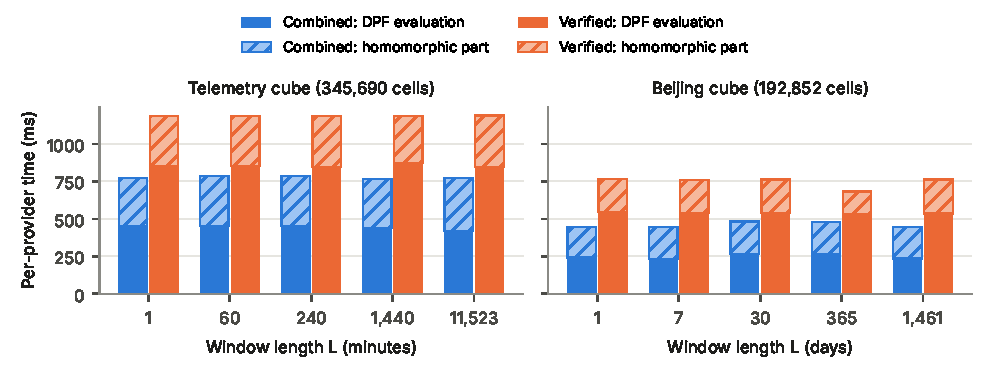
\includegraphics[width=\linewidth]{figures/fig_range_real.pdf}
\caption{Time per cloud for range queries on the two real cubes, by window
length, split into DPF evaluation and homomorphic work.}
\label{fig:real}
\end{figure}

\subsection{Comparison with two alternatives}
\label{sec:baselines}
\para{Describe the two baselines in two sentences each: per-cell keys (no
summed-area table, one key per cell of the box) and a single server (no
non-collusion assumption, encrypted signed-corner vector as the
query).}{bench/bench\_range\_baselines.py.}

\begin{figure}[pos=htbp]
\centering
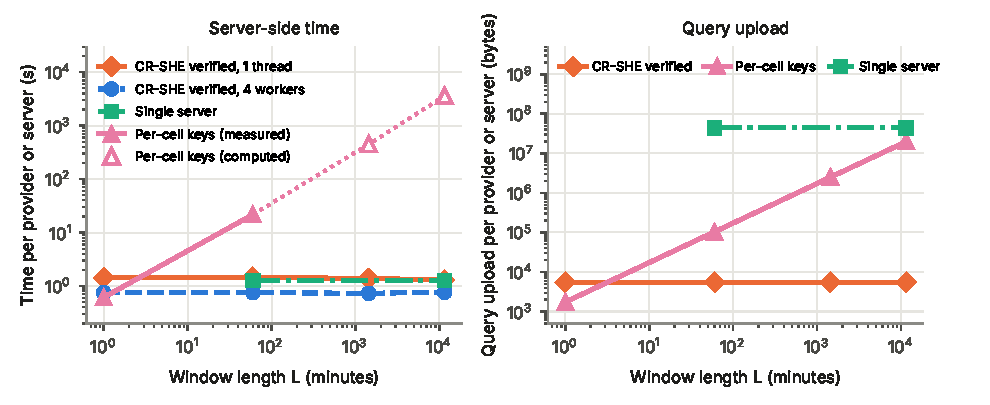
\includegraphics[width=\linewidth]{figures/fig_range_baselines.pdf}
\caption{The same range query answered three ways on one machine: time at the
servers (left) and query upload (right). Open markers are computed, not
measured.}
\label{fig:baselines}
\end{figure}

\para{Without summed-area tables, cost and upload grow with the box, and the
number of keys reveals the box's volume.}{NUMBERS.md, ``Same query three
ways'': per-cell rows. Say which points are computed and how.}

\para{A single server costs about the same server time but needs a query of
tens of megabytes, costs the client encryption time, and cannot use the
check (Remark~\ref{rem:single}). State plainly that the split does not reduce
total server work.}{NUMBERS.md, ``Same query three ways'': single-server rows
and CR-SHE rows.}

\para{Key evaluation parallelises.}{NUMBERS.md: verified, 4 workers.}

\subsection{Detecting wrong answers}
\label{sec:tampereval}
\para{The five injected deviations, one sentence each, then the result: a
stored key misses consistent changes; per-cell stored keys miss a change at
the queried cell; the per-query check catches all.}{Table~\ref{tab:tamper}.
Deviations: add a constant to the value slot; add a uniform vector to the
share; scale the share; change a random cell; change exactly the queried
cell. One cloud deviates, the other is honest.}

\begin{table}[pos=htbp]
\caption{Injected deviations by one of two clouds on the range path:
detected / accepted with a wrong answer.}
\label{tab:tamper}
\centering
\footnotesize
\setlength{\tabcolsep}{3pt}
\begin{tabular*}{\tblwidth}{@{\extracolsep{\fill}}lccccc@{}}
\toprule
Check & Constant & Uniform & Scale & Random cell & Queried cell \\
\midrule
\inputtbl tables/tamper_range.tex
\bottomrule
\end{tabular*}
\end{table}

\subsection{Layouts and cube size}
\label{sec:layouts}
\para{Per-cell stored keys cost about twice the per-query check and still miss
the queried-cell attack; cost grows linearly with the number of cells, so cube
size is what a deployment provisions.}{NUMBERS.md, ``Synthetic cube, layouts''
and ``Cube size''.}

\begin{figure}[pos=htbp]
\centering
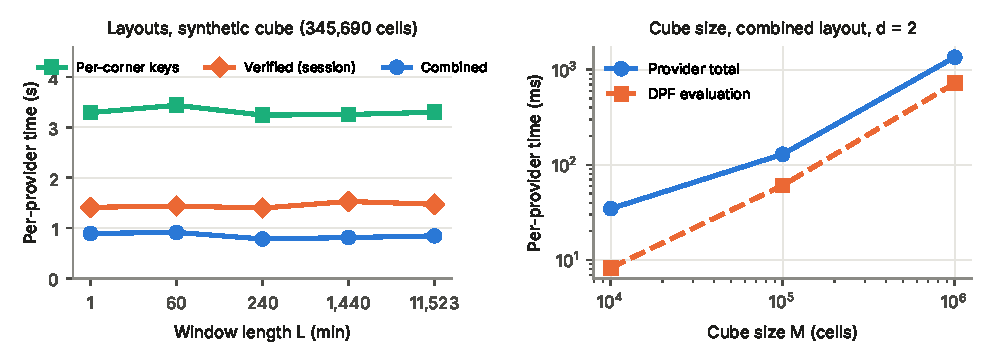
\includegraphics[width=\linewidth]{figures/fig_range_layouts.pdf}
\caption{Time per cloud by layout and window length (left) and by cube size
(right), synthetic cubes.}
\label{fig:layouts}
\end{figure}

% ===========================================================================
\section{Discussion and limitations}
\label{sec:discussion}

\para{What the split buys, and when one server is enough.}{It does not save
server time; it cuts the query from tens of megabytes to kilobytes, removes the
client's encryption work and makes the check sound. A client that can send a
44\,MB query and needs no check can use one server.}

\para{Limitations, honestly.}{Python driver over C++ kernels, one host, no
wide-area measurement (one round trip plus 5.5\,kB up and 132\,kB down per
cloud, so about 0.16\,s at 100\,ms and 20\,Mbit/s, computed); cubes and
templates fixed at setup; cube total below $p$; semi-honest privacy;
non-negative contributions; for $n>2$ the keys are not succinct.}

% ===========================================================================
\section{Conclusion}
\label{sec:conclusion}
\para{Three to five sentences: the problem, the idea, the evidence, one line
of future work.}{Future work: native implementation, cross-region deployment,
succinct keys for $n>2$, several data owners.}

\printcredits

\section*{Declaration of competing interest}
The authors declare that they have no known competing financial interests or
personal relationships that could have appeared to influence the work reported
in this paper.

\section*{Funding}
This research did not receive any specific grant from funding agencies in the
public, commercial, or not-for-profit sectors.

\section*{Data availability}
\para{The authors' statement.}{Both datasets are public
\citep{stafford_2020_environmental,chen2019beijing}. State the terms for the
code.}

\section*{Declaration of generative AI and AI-assisted technologies in the
manuscript preparation process}
\para{The authors' statement, describing what was done for this version.}{
Name every tool and what it did: for example, the reference implementation,
tests, benchmarks and figure scripts written with Claude (Anthropic); the
text written by the authors, with AI help limited to checking numbers,
proofs and references, if that is what happens. Earlier drafts were edited with
ChatGPT and Gemini. Use the journal's required wording at the end.}

\bibliographystyle{model1-num-names}
\bibliography{references}

\end{document}
